% Reference https://www.youtube.com/watch?v=Boltwen-g1g&ab_channel=ChandraHas

\documentclass[11pt,a4paper]{article}

% General
\usepackage[margin=1in]{geometry}
\usepackage[sort&compress,square,numbers]{natbib}
\usepackage{amsmath}
\usepackage{lipsum,times,graphicx,hyperref,cleveref}
\hypersetup{nolinks=true}
\usepackage[labelfont=bf]{caption}
\usepackage{amssymb}

\usepackage{physics}
\usepackage{siunitx}
\usepackage{listings}

% More graphics
\graphicspath{{./images}}
\usepackage[label font={bf, normalsize}]{subfig}
\renewcommand{\thesubfigure}{\Alph{subfigure}}
\usepackage{caption}
\captionsetup{font=normal}
\usepackage{floatrow}
\floatsetup[figure]{subcapbesideposition=top}
\floatsetup[table]{style=plaintop}

\usepackage{titling}
\renewcommand\maketitlehooka{\null\mbox{}\vfill}
\renewcommand\maketitlehookd{\vfill\null}

\title{\vspace{-5cm} {Supplementary material}\\[5mm] 
\textbf{Behavior of weakly adsorbing impurities in flow-through ion-exchange chromatography}}
 
\author{Chase E. Herman, Xuankuo Xu, Steven J. Traylor, Sanchayita Ghose, \and Zheng Jian Li, and Abraham M. Lenhoff}

\date{}

%\renewcommand{\figurename}{Fig.}
\renewcommand{\baselinestretch}{1.33} 
\renewcommand{\thepage}{S\arabic{page}}
\renewcommand{\thetable}{S\arabic{table}}
\renewcommand{\thefigure}{S\arabic{figure}}
\renewcommand{\theequation}{S\arabic{equation}}
%==============================Content=========================
\begin{document}

\begin{titlingpage}
\maketitle
\end{titlingpage}

\begin{figure}[H]
    \centering
    \sidesubfloat[]{\includegraphics[width=0.75\textwidth]%
                    {breakthrough_curves_c_1000_ug_ml}\label{sfig:1 mg/ml}}
    \\
    \sidesubfloat[]{\includegraphics[width=0.75\textwidth]%
                    {breakthrough_curves_c_100_ug_ml}\label{sfig:100 ug/ml}}
    \\
    \sidesubfloat[]{\includegraphics[width=0.75\textwidth]%
                    {breakthrough_curves_c_10_ug_ml}\label{sfig:10 ug/ml}}
    
    \caption{Breakthrough profiles from a simulation of solute loading at \protect\subref{sfig:1 mg/ml} 1 mg/ml, \protect\subref{sfig:100 ug/ml} 100 $\mu$g/ml, and \protect\subref{sfig:10 ug/ml} 10 $\mu$g/ml. Lines correspond to simulations with different $K_{eq}$, which increases by 4 orders of magnitude from left to right. Note that $q_{max}$ was fixed at 100 mg/ml of packed column for all simulations, and the abscissa is on a logarithmic scale.} 
    
    \label{fig:exploratory breakthrough curves - other concentrations}
\end{figure}

\begin{figure}[H]
    \centering
    \vspace{-5.2cm}
    \makebox[\textwidth][c]{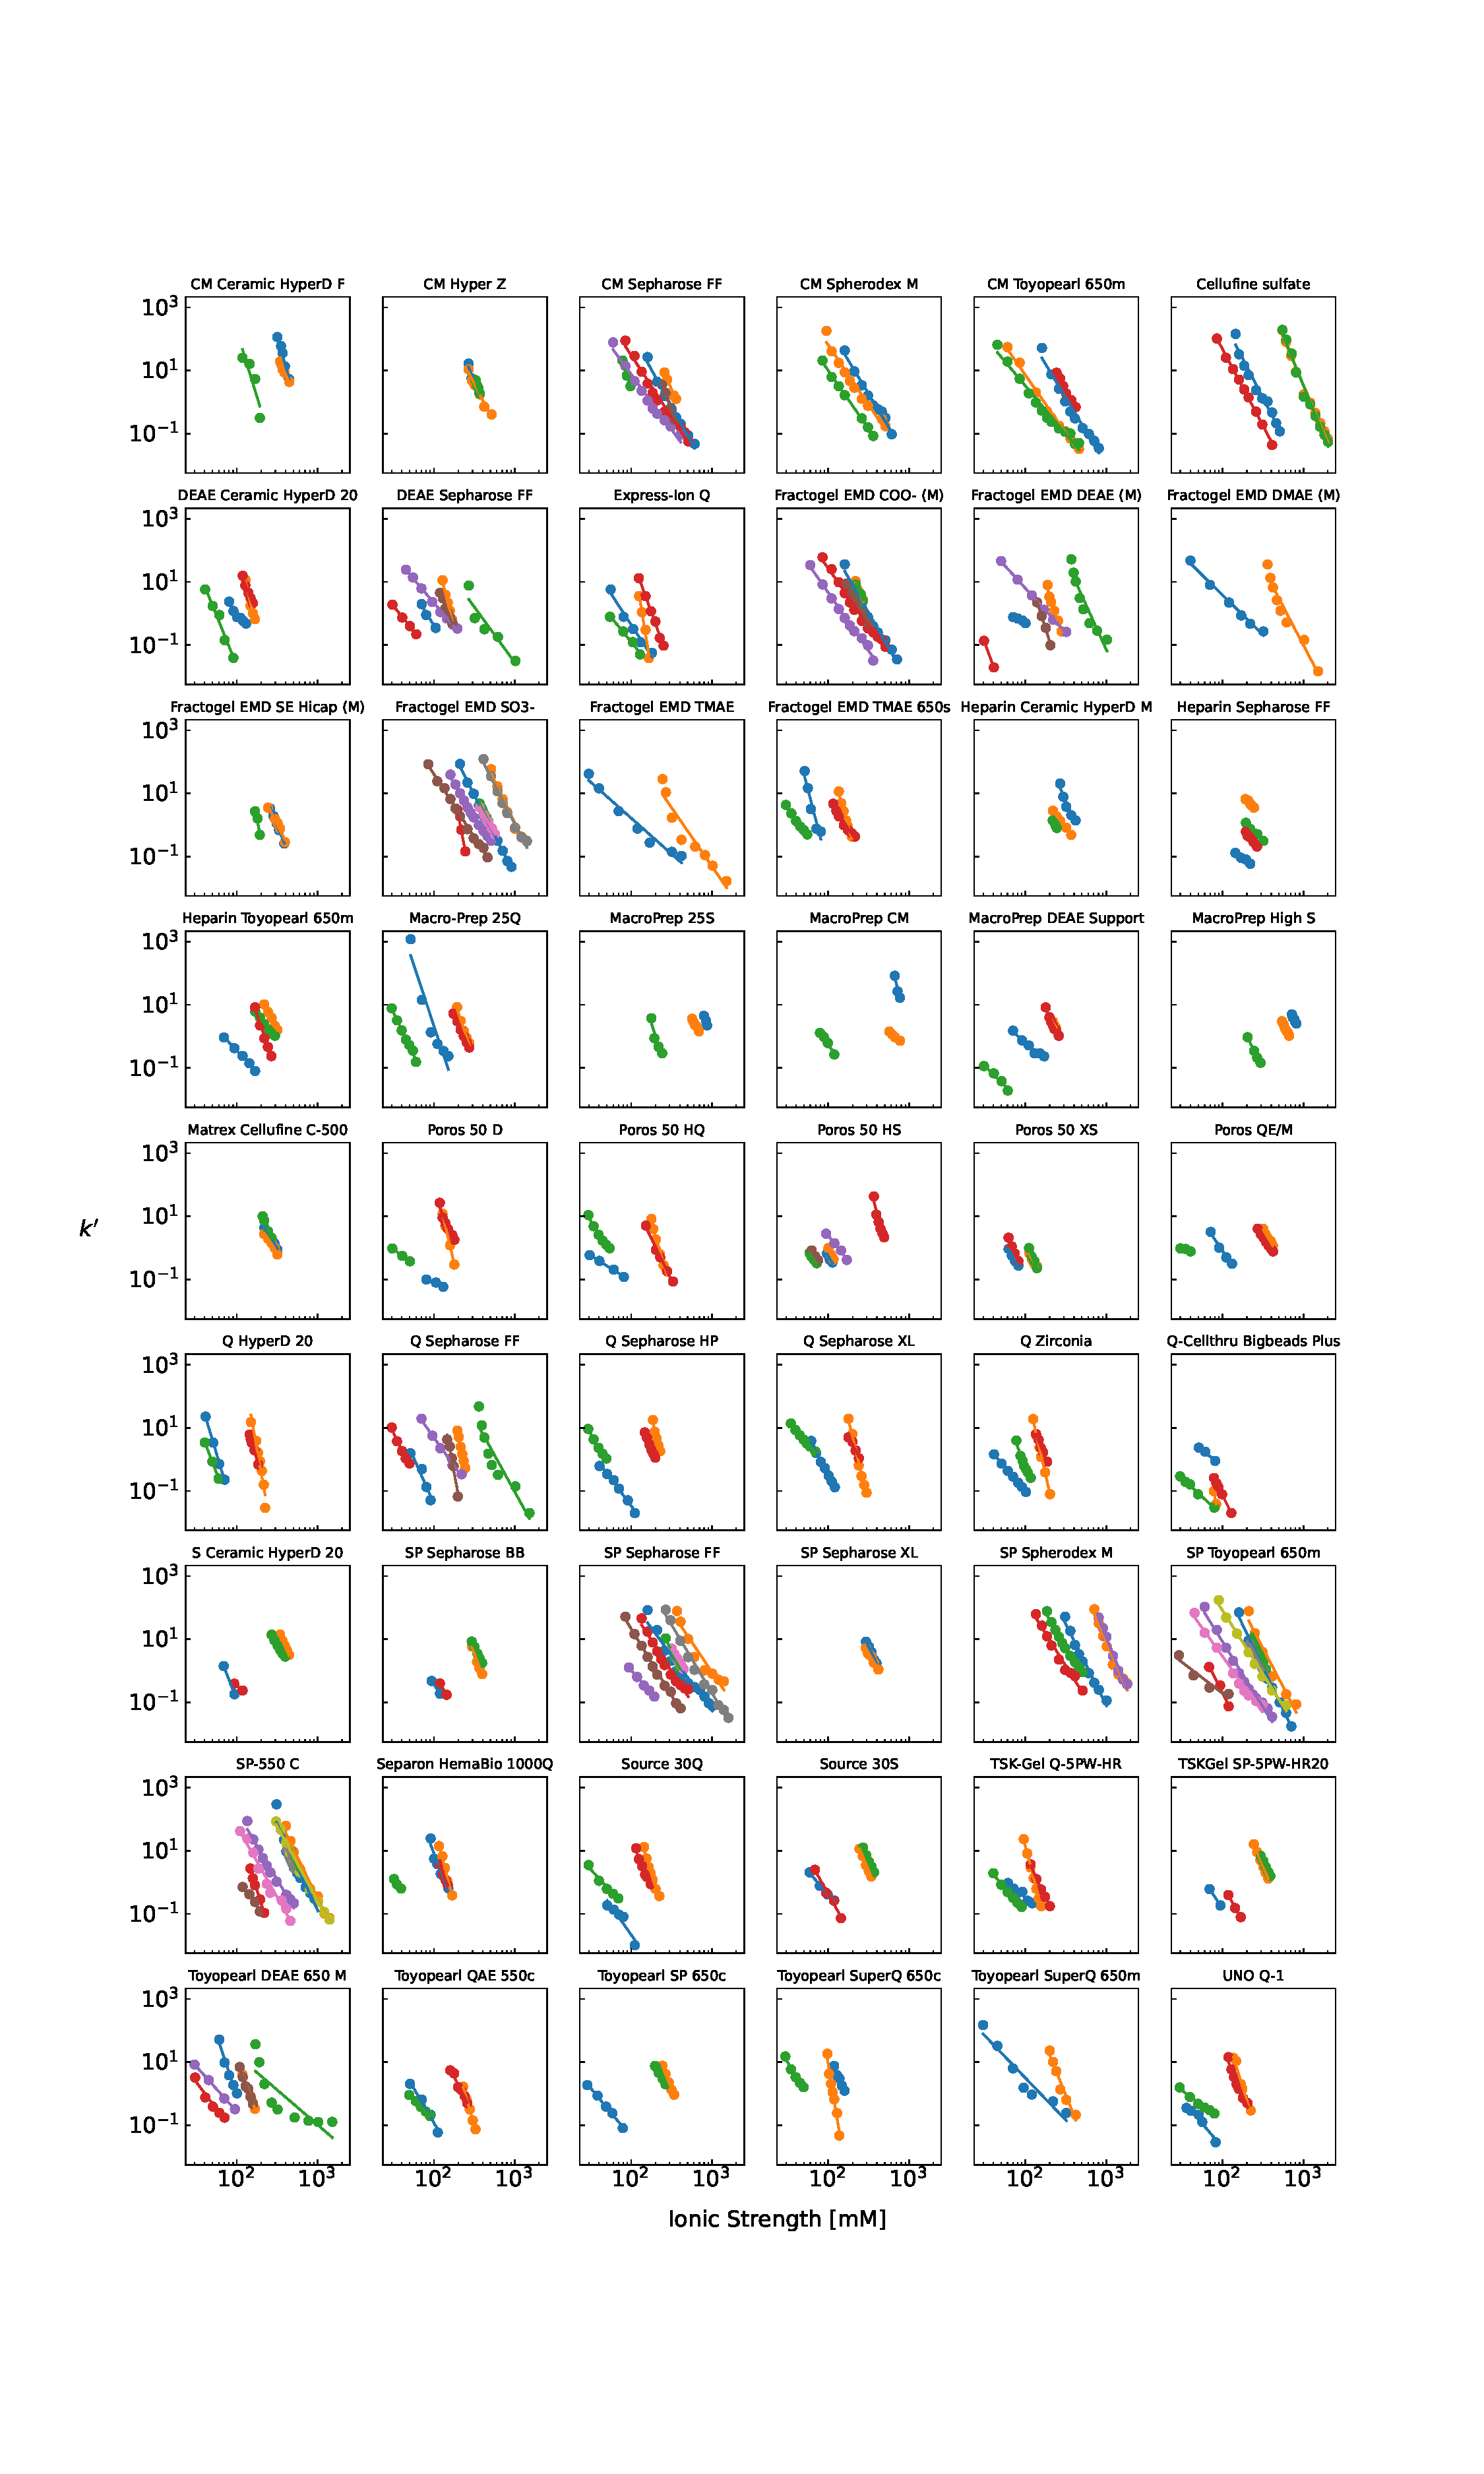
\includegraphics[width=1.2\textwidth]{lit_kprime_data}}
    \vspace{-4cm}
    \caption{Isocratic $k'$ data that were consolidated from the literature. Each series represents a unique protein-pH-resin combination, and lines represent quasi-SDM fits to the data.}
    
    \label{fig:consolidated data}
\end{figure}

\end{document}
